%!TEX root = ./intern_report.tex

\newpage
\subsection{Trailnet: A Classification Network for Autonomous Trail Navigation}

\subsubsection{Trailnet: An Introduction}

\begin{figure}[H]
    \centering
    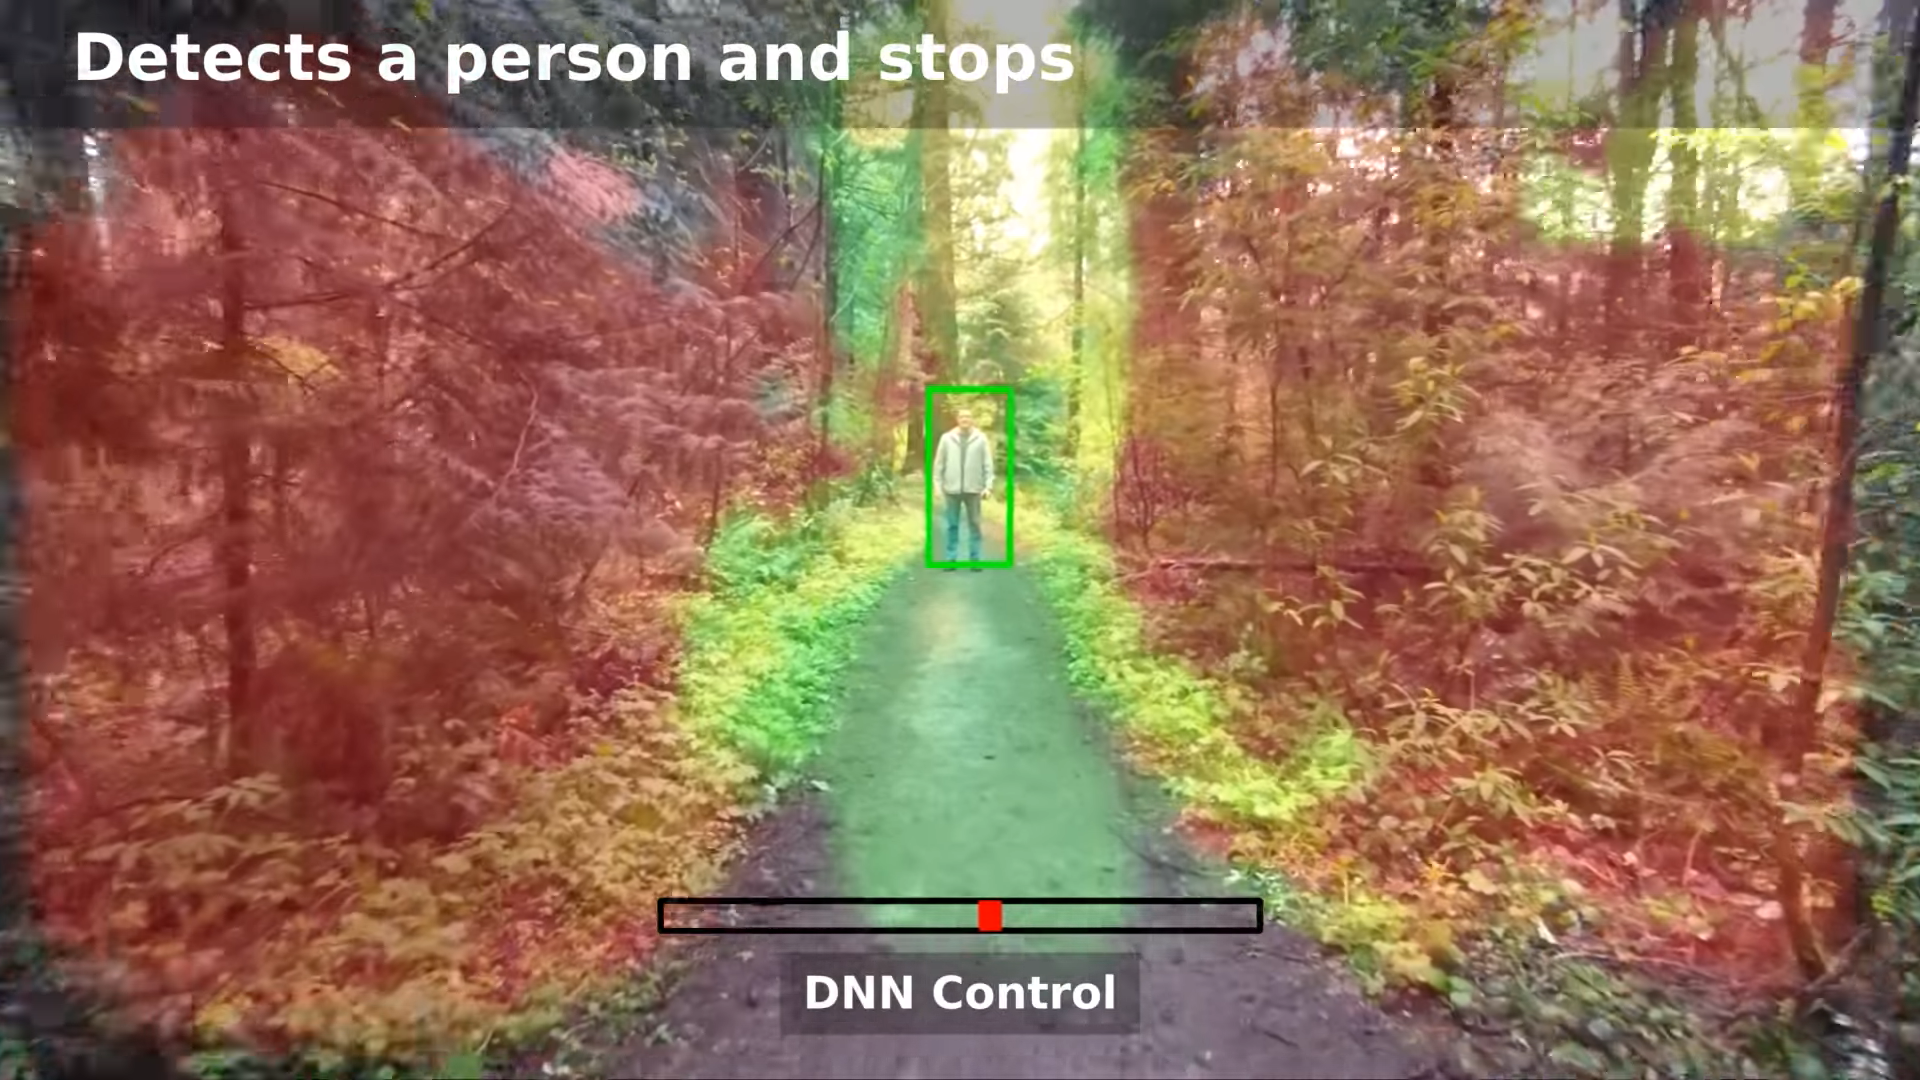
\includegraphics
        [width=10cm]
        {figures/trailnet_redtail_object.png}
    \caption{NVIDIA's Trailnet Navigating a Drone}\vspace{-4mm}
\end{figure}

In 2017, four researchers published a paper titled "Toward Low-Flying Autonomous MAV Trail Navigation using Deep Neural Networks for Environmental Awareness"~\cite{trailNet} (Trailnet paper in short) with the funding of NVIDIA. The paper describes the following:

\begin{itemize}
    \item Merits of approaching autonomous navigation as a classification problem
    \item Architecture of their Trailnet CNN, a modified version of Resnet-18. ~\cite{resnet}
    \item Data collection techniques for the Trailnet CNN
    \item Training Trailnet with a relatively small dataset
    \item Hardware hierarchy and the command flow between cameras, NVIDIA Jetson TX2 ~\cite{jetson_tx2} running ROS and the flight control board.
    \item Usage of YOLO for obstacle detection and algorithm for obstacle avoidance.
    \item Results and observations after flying the quadcopter autonomously in the forest trail for several kilometers.
\end{itemize}

\newpage
\subsubsection{Navigation as Classification}

\paragraph{}
Their model was based on a concept discussed in a 2016 paper %to_cite%,
: approaching autonomous navigation as a classification problem. That is, given an RGB image the CNN would output three probabilities: that of the camera facing left, right or center with respect to the trail. The key advantages in this approach are:

\begin{itemize}
    \item The effect of noise introduced by human errors during data collection on training are minimized due to discretization.
    \item Data collection and labeling is straightforward
    \item Performance can be fine tuned, by adjusting K1 and K2 accordingly. See Figure: \ref{Fig:trailnet_archi}
    \item The depth of the required neural network is less, compared to the regression network that provides similar accurate performance.
    \item Can train the relatively shallow network with a relatively small dataset and shorter training time.
    \item Can be implemented on low powered devices.
\end{itemize}

In the Trailnet paper %to_cite%
They choose Resnet 18 as the basis for their architecture since it is small enough to be run on real time in a power-limited device like Jetson TX2. Resnets (Residual Networks) are special kinds of deep neural network that uses "short circuits" between layer outputs to prevent the problem of vanishing gradients, as a network gets too deep. By employing this technique, researchers have been able to create networks that are thousands of layers deep and still outperform shallower networks. Resnet-18, Resnet-50...etc are popular variants of applying this technique on deep convolutional neural networks.

\paragraph{}
Trailnet is not an RCNN. That is it does not remember past inputs nor correlate current inputs with past and future values for prediction. It is a simple CNN that gives a twist command based on the current image. Input to trailnet is a 320 x 180 x 3 RGB image and the outputs are six softmax nodes connected to the output of a slightly modified resnet-18. The six output layers signify the probability of the given image facing left, center and right and the robot (or UAV) being aligned left, center and right on the path. Weighted (by adjustable constants k1, k2) sum of these probabilities provide the angular twist command, which is used to steer the robot. This additional consideration of alignment, prevents the UAV slowly drifting off the center of the trail and crashing with tree branches near the trail edges. Together, the facing and align probabilities correct the course of the UAV to stay in the center of the path. YOLO and SLAM are used for obstacle avoidance.

\paragraph{}
Data collection was done using a camera rig with 3 cameras facing at three angles (left, center and right). The rig was carried by a person along a forest trail. The video feed from each camera had been then labeled accordingly. Similarly align to left, center and right data has been collected. A pretrained network (previously trained on IDSIA dataset %to_cite%
of 40,000 images) had been fined tuned with this collected data. After training, Trailnet was run with ROS (Robot Operating System) and Caffe on Jetson TX2 on board the UAV. Jetson TX2 receives the video frame from camera, processes it and sends it sends command to the flight controller. 



\subsubsection{Building Trailnet from scratch}

\paragraph{}
One objective of their project was to showcase the capability of NVIDIA's Jetson TX2 high level controller board. Therefore, they had used Caffe framework to build the network and DIGITS framework to train it. However, our key objective in working with this was to build a unified pipeline which all scientists in DATA61 can use. Since most of them were familiar with TensorFlow and since it is the state of the art framework today, I rebuilt the 20-layer network in TensorFlow-Keras and trained it from scratch in CSIRO's supercomputer as I built the pipeline.

% Image: Architecture
\begin{figure}[H]
    \centering
    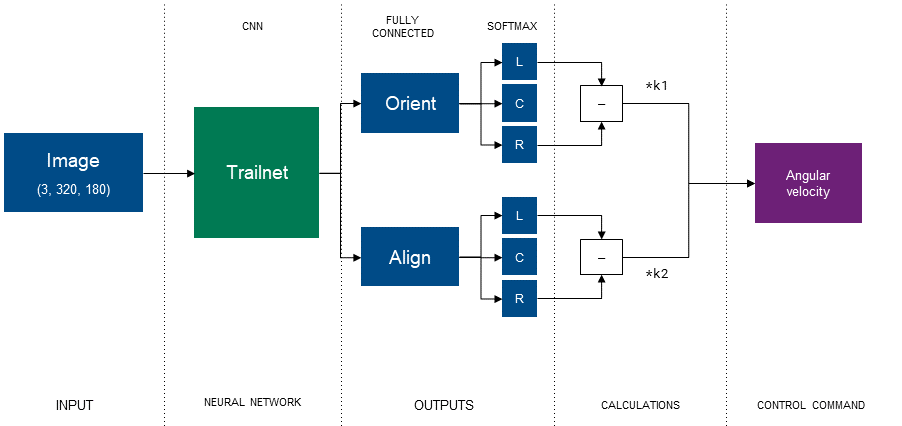
\includegraphics
        [width=16cm]
        {figures/trailnet.PNG}
    \caption{Simplified Trailnet Architecture and Post Processing}\vspace{-4mm}
    \label{Fig:trailnet_archi}
\end{figure}

\subsubsection{Data collection and training Trailnet from scratch}

\paragraph{}
Our goal with this project was to train a robot navigate indoor hallways as a demonstration of our end-to-end pipeline. Hence we mounted three cameras on the robot, facing center, left and right by 30 degrees. We took the robot along the hallways of CSIRO using a remote control and recorded the image stream data as ROS bags. In each hallway, we took the robot on three paths: center aligned, left aligned and right aligned. We then extracted the image stream into an image dataset by taking one image every second (1 fps) from the image stream. The resulting hallway dataset consisted of 120,000 images.

% Image: IDSIA
\begin{figure}[H]
    \centering
    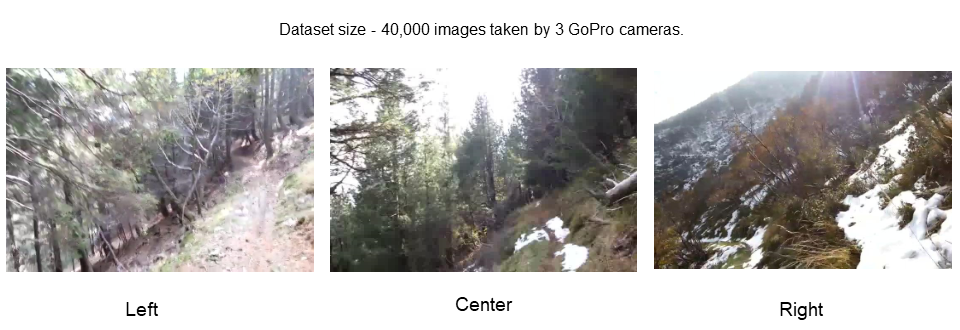
\includegraphics
        [width=16cm]
        {figures/idsia_dataset.PNG}
    \caption{IDSIA Dataset of 40,000 images}\vspace{-4mm}
\end{figure}

% Image: Hallway Dataset
\begin{figure}[H]
    \centering
    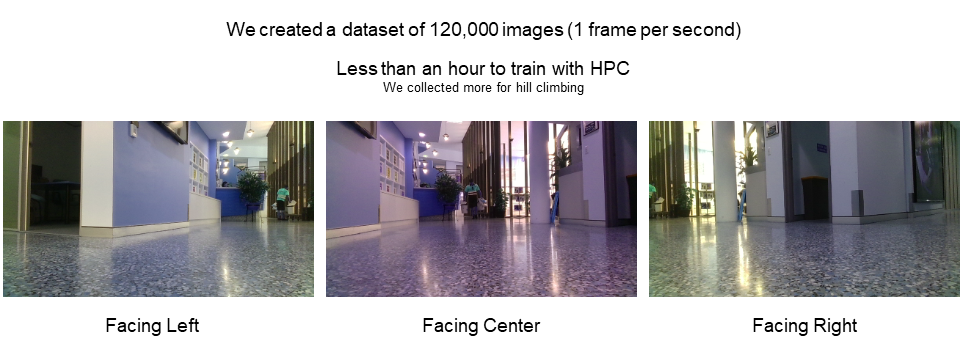
\includegraphics
        [width=16cm]
        {figures/hallway_dataset.PNG}
    \caption{Hallway Dataset of 120,000 images}\vspace{-4mm}
\end{figure}


\paragraph{}
The 120,000 images were stored in the supercomputer and used to train the network. First, align output nodes of Trailnet were frozen and the network (with facing output nodes only) was trained on the IDSIA dataset %to_cite%
 of 40,000 images. Then, the same configuration was trained on the hallway facing dataset. Finally, the facing-output nodes were frozen and the rest (align-output nodes) were trained on the hallway-align dataset.

\paragraph{}
Training the network was a laborious process prone to errors. The supercomputer sessions automatically terminate every few hours, requiring me to stay by the CSIRO provided desktop throughout the process. I stayed overnight for five days alone in the office to train this and the other networks.

\subsubsection{Deployment on a Robot and Testing}

\paragraph{}
The trained model was optimized into a tf-trt graph (See section: \ref{tensorrt}) and executed inside a python based ROS node. The latency was 20 ms, which was enough to process an input image stream at 30 fps during inference. My ROS node also performs necessary calculations and publishes a velocity message (type: geometry\_msgs/Twist)  to a topic that is subscribed by the motor controller and the predictions (type: Float32MultiArray) for debugging. I also designed it in a way that the constants K1, K2 can be tuned by publishing the constants to a topic that is subscribed by the Trailnet ROS node.

\paragraph{}
After setting up this way, the robot was tested for its ability to navigate the hallways autonomously. It's response to external disturbances was checked by kicking the robot in either direction, moving it off the center of the track. K1, K2 constants were tuned to provide the shortest response time while maintaining a steady speed when undisturbed. We also created a visualization technique, where the predictions and commands of the robot can be visualized with the image stream. Following images show the testing process and the corresponding visualization.

% Image: Disturbances
\begin{figure}[H]
    \centering
    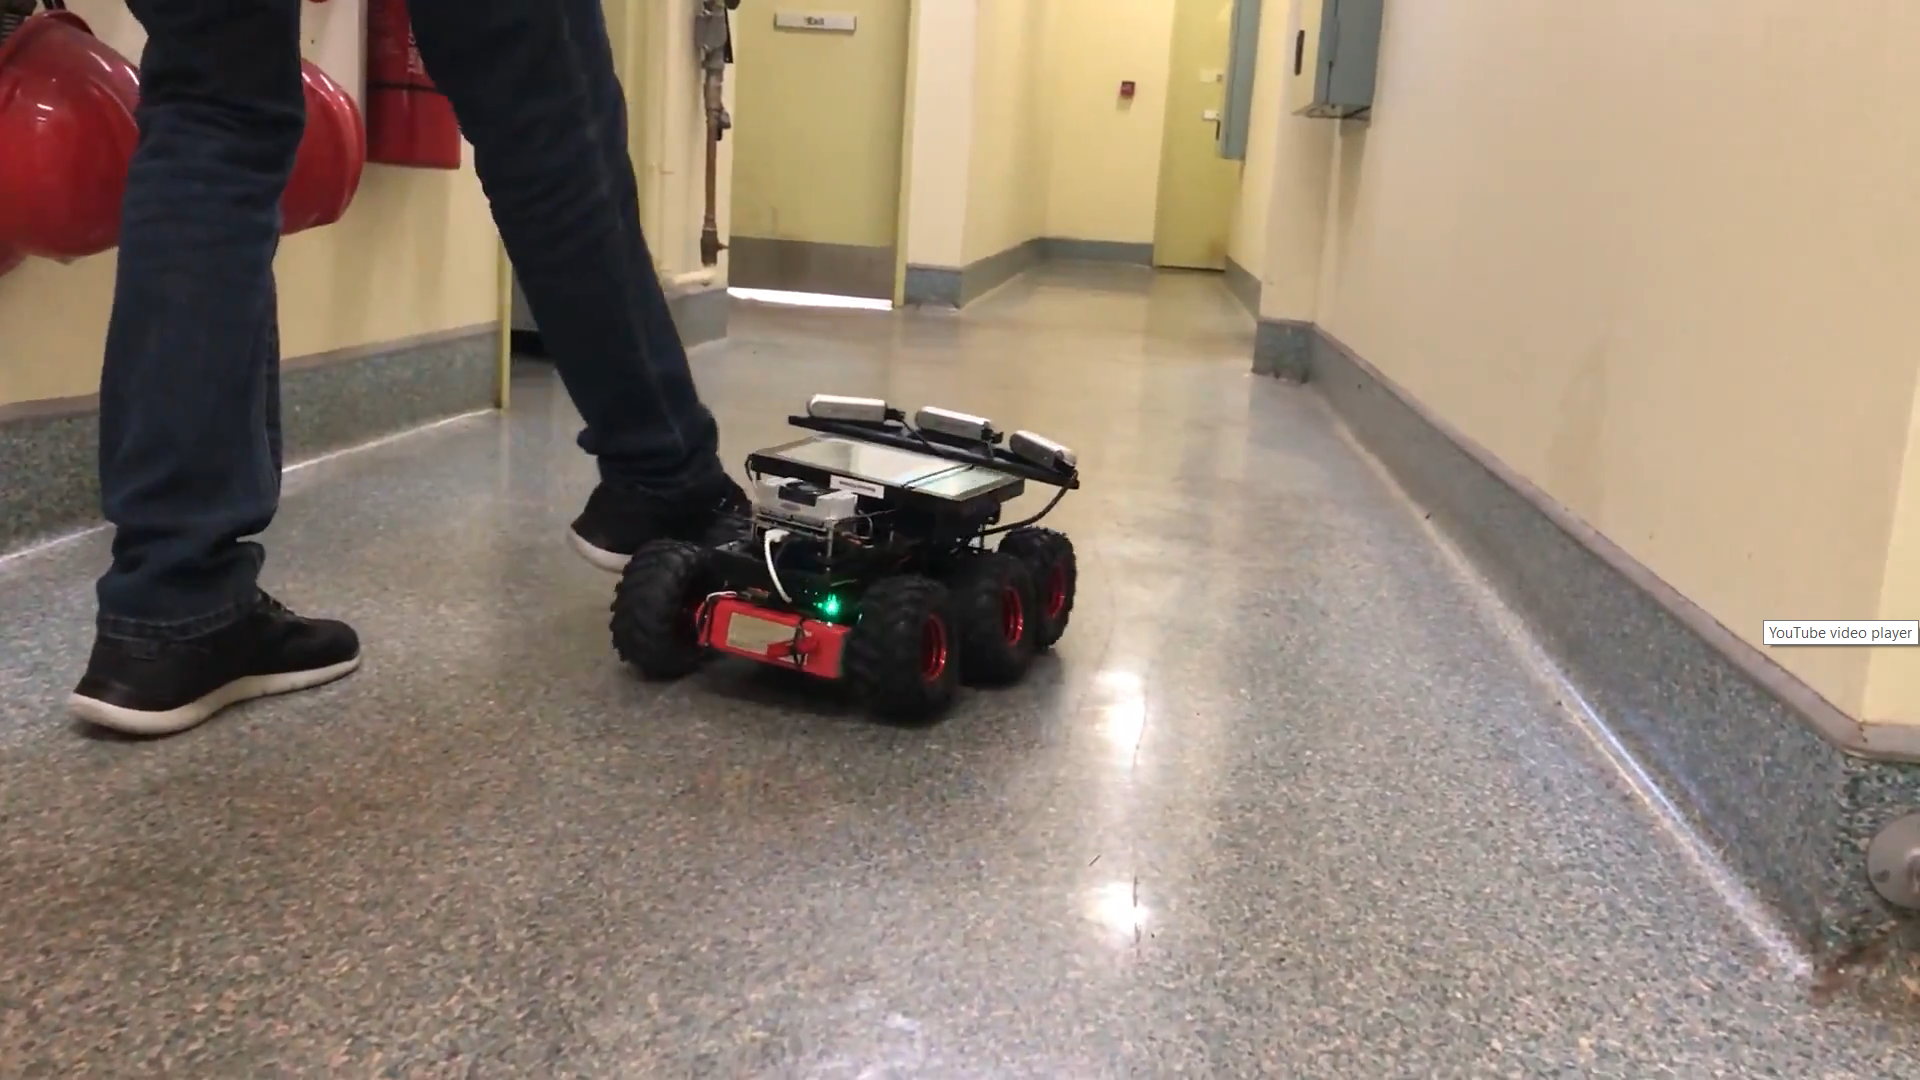
\includegraphics
        [width=.4\linewidth]
        {figures/wallie_self_run.png}
    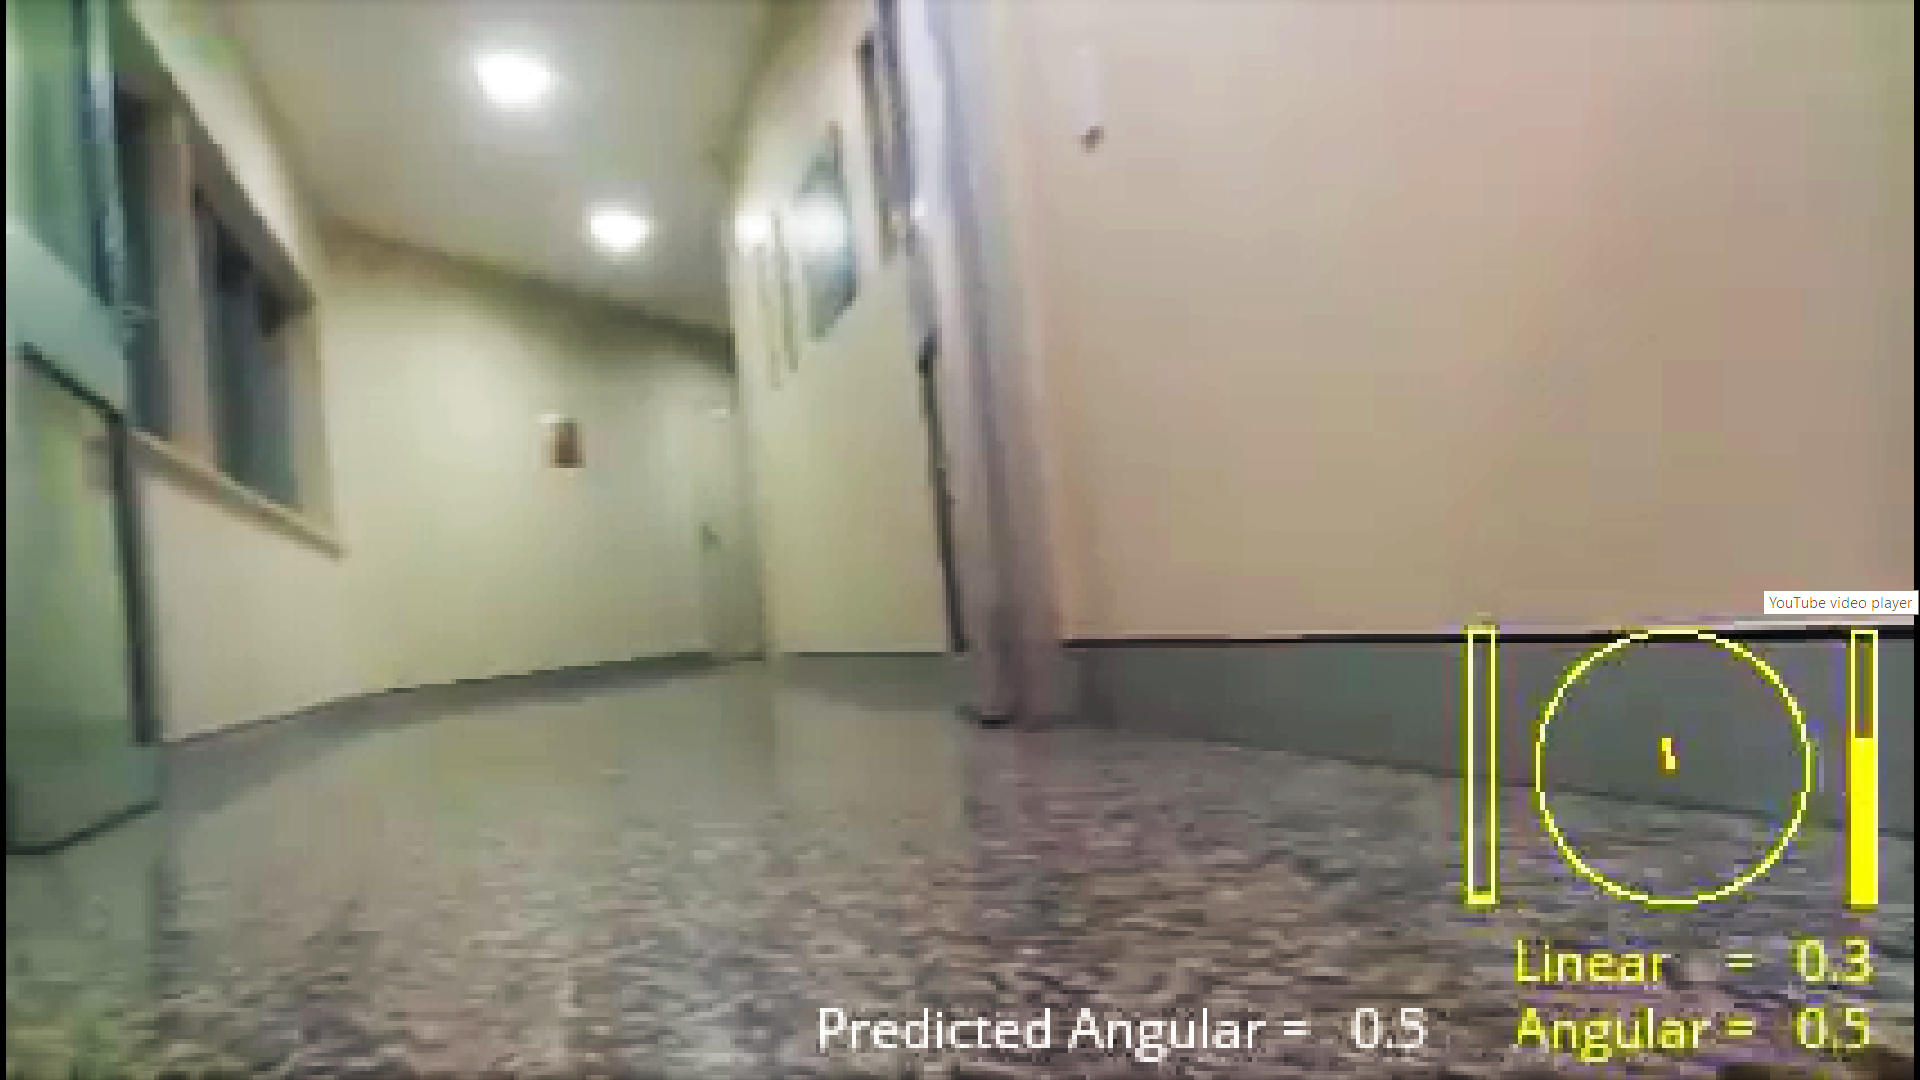
\includegraphics
        [width=.4\linewidth]
        {figures/trailnet_after_kick.png}
    \caption{Our indoor Trailnet CNN reacting to external disturbances}\vspace{-4mm}
    
\end{figure}

\paragraph{}
THe robot was tested in different hallways, including ones from where we did not collect training data. The robot performed remarkably well in cluttered hallways also, showing its robustness %to_cite% 
. In addition to that, the response to 90 degree corners was also remarkable, where the robot smoothly turned to follow the hallway.

% Image: Corners
\begin{figure}[H]
    \centering
    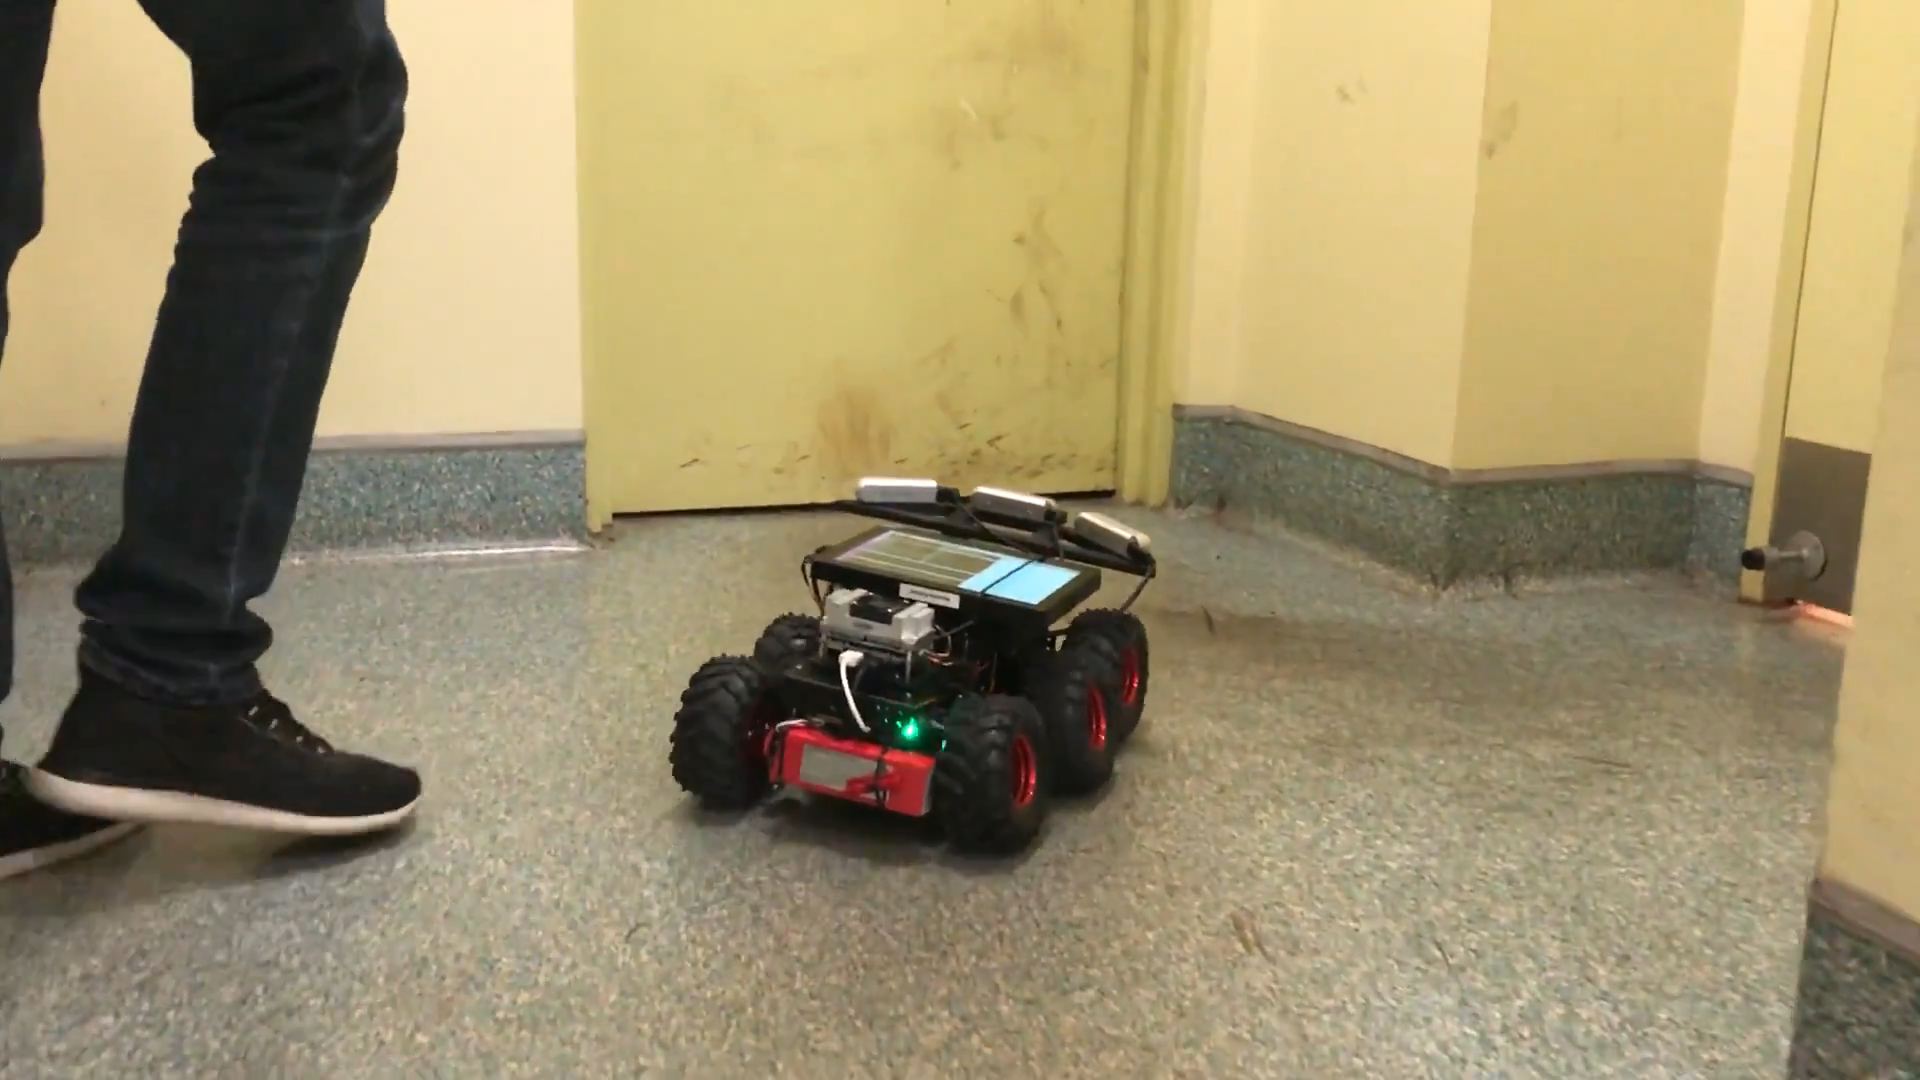
\includegraphics
        [width=6cm]
        {figures/wallie_self_turn.png}
    \caption{Our CNN reacting to corners}\vspace{-4mm}
    
\end{figure}

\paragraph{}
The results were presented to the fellow scientists in a Robotics Reading Group meeting as a demonstration of the end to end pipeline I designed. 